\begin{artengenv}{Szymon Czarnik}
	{How much truth is in stereotypes?}
	{How much truth is in stereotypes?}
	{How much truth is in stereotypes?}
	{Institute of Sociology, Jagiellonian University}
	{Stereotype accuracy is a contentious topic. Part of the problem is that typically stereotypes are generic statements whose truth status is unclear due to the fact that they are ill-defined quantitatively. The article focuses on the epistemic aspect of stereotypical beliefs. In the ongoing debate, I side with those who argue against stereotypes being wrong or inaccurate by virtue of definition alone. I propose that, when possible, stereotype accuracy should be assessed in probabilistic terms by inspecting how likely a generic statement is to be true when applied to individual(s) representative of the relevant group(s). This approach applies equally well to investigating the actual and the perceived accuracy of stereotypes.}
	{stereotypes, stereotype accuracy, epistemology, probabilistic approach.}

\vspace{2\baselineskip}
\lettrine[loversize=0.13,lines=2,lraise=-0.05,nindent=0em,findent=0.2pt]%
{I}{}n this paper, I propose that stereotypes are best understood as generic statements whose truth status is unclear. They are expressed by asserting that ``members of group A have trait T,'' or ``Members of group A are higher/lower on trait T than members of group B.'' Such utterances lack proper quantification and invite alternative interpretations. One such interpretation is that stereotypes speak of all group members without exception which leads to the idea that stereotypes should be considered false by definition, which in turn leads to the opposition to stereotype accuracy research as, at best, a misguided endeavor. This opposition, however, is unfounded on epistemic grounds once we explicitly recognize generic nature of stereotypes. Thus after outlining the long-lasting debate, I proceed to discuss the problems inherent in measuring the accuracy of stereotypes, and then advocate a probabilistic approach, i.e. assessment of probabilities that individuals conform to the generic rule posited by a stereotype. As a practical illustration, I show a number of such probabilistic assessments based on data from representative samples. Finally, I propose that the very same probabilistic approach should be used to directly investigate how accurate people perceive their own stereotypes to be. This in turn would provide an easy and straightforward method of comparing perceived and actual accuracy of stereotypes, acknowledging a possibility that stereotypical perceptions may both over- and underestimate actual differences.


\begin{center}
$ {\ast}\,{\ast}\,{\ast} $
\end{center}


A scholarly dispute over stereotypes is to no small extent a semantic issue. The problem is that a typical stereotype assumes a form of what \textit{The Stanford Encyclopedia of Philosophy} calls a generic, i.e. a statement which expresses a generalization ``but unlike quantified statements, [...] do[es] not carry information about how many members of the kind or category have the property''
%\label{ref:RNDGhTTUrWVcB}(Leslie and Lerner, 2016).
\parencite[][]{leslie_generic_2016}. %
 ``Some men are taller than some women'' is certainly a true statement. Equally certainly, ``All men are taller than all women'' is a false statement. But the case is that when you hear anybody compare the height of men and women, it will be in the form of a generic ``Men are taller than women.'' A quantitative indeterminacy of such an utterance will either be construed to be vaguely true and will be silently approved, or will invite a dispute and be contested.

\enlargethispage{.7\baselineskip}
In daily life conversations, calling somebody's remark a stereotype is surely a form of criticism. In common parlance, as well as in vast sociological and psychological literature, the term ‘stereotype' implies untruth, or inaccuracy of the assertion. A general statement like ``Scots are cheap'' may be picked apart as untrue in the sense that on average Scots are no more stingy than members of any other ethnic group. Or, even if the statement had some kernel of truth in it, one could be brought to task for inaccurately applying it to pass a judgment on a particular individual who may happen not to conform to this general rule.\footnote{Far from being limited to stereotypical beliefs, the problem of group-to-individual generalizability may pose a serious threat to scientific research involving human subjects
%\label{ref:RNDTlfuAJ4ACM}(Fisher, Medaglia and Jeronimus, 2018).
\parencite[][]{fisher_lack_2018}.%
} Apart from being misguided epistemologically, the utterance may also be criticized on moral grounds as an attempt at a wholesale vilification of a certain group of people. Thus the presumed wrongness of stereotypes may consist in epistemic and/or moral failure 
%\label{ref:RNDo2Xq32gcjA}(Beeghly, 2014).
\parencite[][]{beeghly_seeing_2014}. %
 It is solely the former aspect of stereotypes that we shall be concerned with here.\footnote{Some authors reduce stereotypes to the epistemic aspect alone. Thus Banaji claims that ``[f]rom the earliest use of the term in psychology, stereotypes have been regarded as the cognitive (thought) as opposed to the affective (feeling) component of mental representations of social groups. As such, the construct is tied to but differentiated from the concept of attitude, preference, or liking as well as the concept of discrimination'' 
%\label{ref:RNDHS9MlJPRnC}(Banaji, 2001, p.15101).
\parencite[][p.15101]{banaji_stereotypes_2001}. %
 }

\section{Resistance to research on stereotype accuracy}
Before we proceed further it should be acknowledged that, for a good reason, the ethical aspect looms large in the scholarly literature on the topic. In psychology, stereotypes are studied as cognitive components of prejudice, which may be brought about by and contribute to inter-group hostility
%\label{ref:RND4lT4IExI0w}(Bar-Tal, 1989);
\parencite[][]{bar-tal_delegitimization_1989}; %
 in sociology, they are recognized as a device that may adversely affect targeted groups by means of self-fulfilling prophecy 
%\label{ref:RNDq8zLOYvax2}(Merton, 1948);
\parencite[][]{merton_self-fulfilling_1948}; %
 in criminology, they are discussed in the context of racial/ethnic profiling in police operations 
%\label{ref:RNDFHF118jk89}(Schauer, 2003);
\parencite[][]{schauer_profiles_2003}; %
 in historical studies, they are investigated as part and parcel of totalitarian propaganda 
%\label{ref:RND3zPpNfYi3y}(Werth, 2011; USHMM (United States Holocaust Memorial Museum),
\parencites[][]{werth_dekulakisation_2011}[][]{ushmm_united_states_holocaust_memorial_museum_defining_nodate}%
; in economics, they are incorporated in models of statistical discrimination in the labor market 
%\label{ref:RNDgoefvun65q}(Arrow, 1971; Phelps, 1972).
\parencites[][]{arrow_theory_1971}[][]{phelps_statistical_1972}. %
 It goes without saying that after Adorno had linked stereotypic thinking with fascist belief systems the concept became even more anathema 
%\label{ref:RNDHdzxZxrjhG}(Jones and Colman, 2001).
\parencite[][]{jones_stereotypes_2001}.%


It is then easy to see why the very idea of considering stereotype accuracy has been frowned upon. Being a lively research field until around mid-1950s, in later years accuracy research nearly ceased to exist
%\label{ref:RNDEUrLdTnpLb}(Jussim, 2012).
\parencite[][]{jussim_social_2012}. %
 Recognized harmful implications of stereotypes made most researchers extremely reluctant to lend them any credibility for fear of promoting any sort of prejudice. In most of the writings on stereotypes, this reluctance tended to be implicitly transformed into a non-sequitur assumption that ``if stereotypes are associated with social wrongs, they must be factually wrong'' 
%\label{ref:RNDbpqmbn3un6}(Jussim et al., 2009, p.199).
\parencite[][p.199]{jussim_unbearable_2009}. %
 This conflation was brought up and chastised as early as 1965 by Roger Brown who opined that it was a disingenuous device by means of which the social psychologist ``perverted his science to achieve a moral purpose'' 
%\label{ref:RND5F22AusjVZ}(Stroebe and Insko, 1989, p.5).
\parencite[][p.5]{stroebe_stereotype_1989}.%
\footnote{We encounter a similar sentiment even earlier in a seminal book 
%\label{ref:RND0GRWHWvKN6}(Allport, 1954, p.87):
\parencite[][p.87]{allport_nature_1954}: %
 ``we find social scientists who overhastily reject the very possibility of racial, national, or group differences of any appreciable or fundamental order. Some of them do so on the basis of charitable motives, but the evidence they offer is usually fragmentary''. He even goes as far as to urge researchers to investigate ``all the facts we can get to evaluate the alleged claim that a hated group merits hostility—that its evil reputation is well deserved'' 
%\label{ref:RNDVZBwqFCsZG}(Allport, 1954, p.104)
\parencite[][p.104]{allport_nature_1954}%
—an utterance that in the present day and age would likely bring upon him a charge of ``blaming the victim''. } Still thirty years later, going against the tide, the editors of \textit{Stereotype Accuracy. Toward Appreciating Group Differences} forewarned in the preface:

\myquote{
It is not easy to do research on stereotype accuracy, for both scientific and political reasons […]. The intellectual content of this book commits multiple heresies […] the idea that stereotypes may sometimes have some degree of accuracy is apparently anathema to many social scientists and laypeople. Those who document accuracy run the risk of being seen as racists, sexists, or worse
%\label{ref:RNDt9JkRYIBWn}(Lee, Jussim and McCauley, 1995, p.xiii).
\parencite[][p.xiii]{lee_stereotype_1995}.%
\footnote{Indeed, stereotypes acquired such a contemptible connotation that it became a useful strategy for overbearing intellectuals to attach the term to any commonsensical statement they found unpalatable. As Thomas Sowell observed, ``the very conception of testing beliefs against reality is attacked by such things as deconstruction, cultural relativism, and the practice of describing uncongenial conclusions as ‘perceptions' or ‘stereotypes' and attributing ‘false consciousness' to those who hold them'' 
%\label{ref:RNDjeSrl3zJq4}(Sowell, 1995, p.244).
\parencite[][p.244]{sowell_vision_1995}. %
 }
}


Needless to say, authors go to great lengths to explicate why the slur is utterly unfounded.

\section{Ambiguity about truth status of stereotypes}
Hostility toward stereotype accuracy reported by Jussim et al. notwithstanding, one should recognize that from the very outset there was a lot of ambiguity about the truth status of stereotypes. Two of the most seminal pieces on stereotypes, viz. Part III of \textit{Public Opinion} by Walter Lippmann (credited with introducing the concept in 1922), and \textit{The Nature of Prejudice}
%\label{ref:RNDZbhHfsclbw}(1954)
by Gordon W. Allport
\parencite*[][]{allport_nature_1954} %
are case in point. They both consider stereotype formation as a natural and inevitable process taking place in human mind when people try to make sense of a limited amount of information. Likewise, they both admit that beliefs about groups may be correct to different degrees. Thus, for example, Lippmann 
%\label{ref:RNDBg29dJm9cU}(1998, p.90)
\parencite*[][p.90]{lippmann_public_1998} %
 observes:

%\enlargethispage{1\baselineskip}
\myquote{
Were there no practical uniformities in the environment, there would be no economy and only error in the human habit of accepting foresight for sight.\footnote{Lippmann construed stereotypes as preconceptions that guide and organize our perception. } But there are uniformities sufficiently accurate, and the need of economizing attention is so inevitable, that the abandonment of all stereotypes for a wholly innocent approach to experience would impoverish human life.
}

But having admitted this much, he offers a very telling example of what he considers to be a perfect stereotype. He invokes Aristotle's infamous defense of slavery in Book I of \textit{Politics}. Therein the philosopher instructs his readers that nature created the bodies of slaves and free men different from each other: the former fit for servile labor, the latter for civil life. Utter nonsense as it is, notes Lippmann, training Greeks to see slaves as slaves by nature was presumably the only ``righteous'' justification of the institution one could offer. He then sums up Aristotle's persuasion strategy:

\myquote{
Each slave holder was to look upon his chattels as natural slaves. When his eye had been trained to see them that way, he was to note as confirmation of their servile character the fact that they performed servile work, that they were competent to do servile work, and that they had the muscles to do servile work.

This is the perfect stereotype. Its hallmark is that it precedes the use of reason; is a form of perception, imposes a certain character on the data of our senses before the data reach the intelligence […]. There is nothing so obdurate to education or to criticism as the stereotype. (p.98)
}

In a similar fashion Allport
%\label{ref:RNDoannRVTDJI}(1954, pp.189–190),
\parencite*[][pp.189–190]{allport_nature_1954}, %
 while conceding that some stereotypes ``need not be altogether false'', points to the fact that there are as well some that ``are totally unsupported by facts'' and it's possible for them ``to grow in defiance of all evidence.''

%\enlargethispage{1\baselineskip}
\section{Are stereotypes untrue by definition?}
There is not one agreed upon definition of stereotypes. Probably the shortest and most general definition of stereotypes as ``category-based knowledge'' was provided \textit{en passant} by Macrae and Quadflieg in a chapter on perceiving people
%\label{ref:RND3OKSCJItmJ}(Macrae and Quadflieg, 2010, p.428).
\parencite[][p.428]{macrae_perceiving_2010}. %
 In the social context, such categories would predominantly be groups of people sharing a certain salient characteristic. Naturally enough, most definitions add certain qualifications, of which the one pertinent to our topic is whether stereotypes are necessarily untrue, or inaccurate. As Stroebe and Insko 
%\label{ref:RNDBPlnl0NzfU}(1989)
\parencite*[][]{stroebe_stereotype_1989} %
 point out, stereotypes have often been defined as ``incorrect generalizations''; they were variously meant to be ``relatively unresponsive to external reality'' 
%\label{ref:RNDg8YZLD95aE}(Klineberg, 1951),
\parencite[][]{klineberg_scientific_1951}, %
 ``exaggerated'' 
%\label{ref:RNDik6HuiuzNF}(Allport, 1954),
\parencite[][]{allport_nature_1954}, %
 ``biased'' 
%\label{ref:RNDf006k8PUql}(English and English, 1958),
\parencite[][]{english_comprehensive_1958}, %
 ``generally invalid'' 
%\label{ref:RNDI3CYnMSqCL}(Miller and Turnbull, 1986)
\parencite[][]{miller_expectancies_1986}%
\footnote{It is ironic and telling that defining stereotypes as generally invalid, Miller and Turnbull quote Ashmore and Del Boca 
%\label{ref:RNDP7GpDYrS3x}(1981)
\parencite*[][]{hamilton_conceptual_1981} %
 who, in the very paper quoted, explicitly advocated accuracy-neutral definition: ``Stereotypes have been defined as ‘bad' for one or a combination of the following reasons: A stereotype is a set of beliefs that is incorrectly learned, overgeneralized, factually incorrect, or rigid [...]. While stereotypes may well have any or all of these characteristics, the proposed sources of ‘badness' should not be incorporated into the definition of the term ‘stereotype''' 
%\label{ref:RNDKNEzt09O1t}(Miller and Turnbull, 1986, p.16).
\parencite[][p.16]{miller_expectancies_1986}.%
}, ``oversimplified'' 
%\label{ref:RNDIW40zgJp1x}(Koleser, 2008),
\parencite[][]{koleser_stereotyping_2008}, %
 ``over-generalized'' 
%\label{ref:RNDgh0MDtr3mm}(Wikipedia, 2020),
\parencite[][]{wikipedia_stereotype_2020}, %
 etc.\footnote{Other characteristics, frequently added, have rendered stereotypes negative, resistant to change, and disindividualized (shared within a particular social environment).} However, Jussim et al. 
%\label{ref:RNDWPSqDkaPbN}(2009)
\enlargethispage{-.5\baselineskip}%
\parencite*[][]{jussim_unbearable_2009} %
 supplied a cogent argument against such defining away of stereotype's accuracy. The argument is two-fold as, logically, there are only two possible interpretations of the assertion that all stereotypes are inaccurate. First reading is that all beliefs about groups are stereotypes and they are all wrong. As a matter of fact, hardly anybody subscribes to such a claim. It is quite obviously self-defeating because if it was true, any meaningful discussion about groups of people would \textit{ipso facto} be impossible. Second interpretation is that not all beliefs about groups are wrong and we call stereotypes only those that are.\footnote{This in fact was the position taken by Allport who made an explicit distinction between stereotypes (distorted beliefs) and group traits (real differences between groups): ``If [an image of a category] is a generalized judgment based on a certain probability that an object of the class will possess a given attribute, we would not call the judgment a stereotype'' 
%\label{ref:RNDdBClyv6yLF}(Allport, 1954, p.189).
\parencite[][p.189]{allport_nature_1954}. %
 And then: ``We can distinguish between a valid generalization and a stereotype only if we have solid data concerning the existence of (the probability of) true group differences'' 
%\label{ref:RNDyBG6R329S4}(Allport, 1954, p.192})
\parencite[][p.192]{allport_nature_1954}.}
 The problem with this approach is that it is inconsistent with the actual practice of research on stereotypes. It necessitates that the first step in stereotype research should be to demonstrate that the belief under investigation is indeed factually wrong. Otherwise, it would plainly not be a stereotype study. However, in practice that first step is typically skipped, the burden of proof is left untouched and it is simply assumed that the belief is false.\footnote{The reason for this
% , Jussim et al. 
%\label{ref:RNDnGvl9HW20z}(2016, p.33)
%\parencite*[][p.33]{jussim_stereotype_2016} %
% surmise,
 is that ``social psychologists once so firmly believed in stereotype inaccuracy, that declaring stereotypes to be inaccurate did not even require a reference!'' \parencite[][p.33]{jussim_stereotype_2016}} Jussim et al. 
%\label{ref:RNDlkKeugSyNP}(2016, p.32)
\parencite*[][p.32]{jussim_stereotype_2016} %
 dub this phenomenon ``The Black Hole at the Bottom of Many Declarations of Stereotype Inaccuracy''. By means of exemplification, they quote a passage from a world-renowned social psychology handbook stating that ``[t]o stereotype is to allow those pictures [i.e. our mental images of external reality] to dominate our thinking, leading us to assign identical characteristics to any person in a group, regardless of the actual variation among members of that group'' 
%\label{ref:RNDfTxHUaw0Cl}(Aronson, 2011, p.309).
\parencite[][p.309]{aronson_social_2011}. %
 As they are quick to notice, Aronson ``does not cite anything to support such an extreme claim because he cannot. After nearly 100 years of empirical research on social stereotypes, there is not a single study that has reported a single person who believes all members of any group have identical characteristics'' 
%\label{ref:RND2AGqqANLO3}(Jussim et al., 2016, p.33).
\parencite[][p.33]{jussim_stereotype_2016}.%

\enlargethispage{.5\baselineskip}
Still another more serious problem is that stereotype itself is a categorical concept, and since beliefs about groups may be located anywhere on the continuum between blatant falsehood and clear truth, to categorize a statement as a stereotype one needs to choose a cut-off point—a purely arbitrary decision. To be sure, any academic might argue that the cut-off point should simply be 100\% true; that a given stereotype, e.g. that men are taller than women, may be considered true only if each and every man is taller than any woman.\footnote{As the above quote from Aronson shows, this line of reasoning is routinely employed to demonstrate that stereotypes are false. } But then one is left wondering how many of the propositions based on social-scientific studies would hold their ground for more than five seconds when faced with such an absurdly high standard of truth.\footnote{As a matter of fact, Jussim et al.
%\label{ref:RNDCjdzj1pbxk}(2016)
\parencite*[][]{jussim_stereotype_2016} %
 make a point of demonstrating that correlations between stereotypic beliefs and actual data on group characteristics are substantially higher than those observed in most studies in social psychology. } As it is, it stands to reason that this Gordian knot should be cut—as Jussim et al. propose—by agreeing on an accuracy-neutral definition of stereotype, making it an umbrella term for all beliefs about groups, and leaving it open to empirical investigation how much trust we can put in any of them.\footnote{For the very same reason, it would be wise not to define stereotypes as a type of commonly held beliefs. Again, the commonness of a particular stereotype could be determined empirically. At one extreme, one could even speak of a single person having a peculiar stereotype of a given group. Thus Jussim et al. 
%\label{ref:RNDbYMASiaKUc}(2016)
\parencite*[][]{jussim_stereotype_2016} %
 distinguish between individual and consensual stereotypes. Apart from that, the problem of measuring belief's accuracy is completely independent of how many people really believe~it.}
 Obviously, as they explicitly make clear, ``rejection of defining stereotypes as inaccurate is not equivalent to defining them as accurate.'' 
%\label{ref:RNDTNbw7p1vbo}(Jussim et al., 2016, p.202).
\parencite[][p.202]{jussim_stereotype_2016}. %
 A good example of an accuracy-neutral definition is the one provided by Ashmore and Del Boca 
%\label{ref:RNDdmXZ9YYXlE}(1981, p.16),
\parencite*[][p.16]{hamilton_conceptual_1981}, %
 wherein the core meaning of a stereotype (i.e. shared by all scholars dealing with the subject) makes it simply a ``set of beliefs about the personal attributes of a group of people''. This definition is then followed by a series of arguments why stereotypes should not be treated as intrinsically ``bad''.

\enlargethispage{.5\baselineskip}
\section[Problems in measuring the accuracy of stereotypes]{Problems in measuring the accuracy of stereotypes\footnote{It should be stressed that what I am interested in here is the extent to which stereotypical judgments as such are correct. It is a related but separate issue whether the process by which people arrive at their judgments is correct. For example, someone may arrive at a correct estimate of honesty in a given group of people, even though he overestimates honesty of people in general while underestimating honesty of that particular group relative to general public. See
%\label{ref:RNDq1DptTqYi9}(Jussim et al., 2016)
\parencite[][]{jussim_stereotype_2016} %
 for a discussion of processual models of judgment by Cronbach 
%\label{ref:RNDqEAFrZBRPd}(1955)
\parencite*[][]{cronbach_processes_1955} %
 and Kenny 
%\label{ref:RNDlQ5sgtU4cA}(Kenny, 1994).
\parencite*[][]{kenny_interpersonal_1994}. %
 }}
Assessing stereotype (in)accuracy involves three obvious steps
%\label{ref:RNDr97wsTQtKY}(Jussim, Crawford and Rubinstein, 2015):
\parencite[][]{jussim_stereotype_2015}:%


\begin{enumerate}
\item Eliciting person's belief about certain group(s) with regard to a particular characteristic.
\item Identifying criteria, i.e. relevant reference data on the target group.
\item Comparing beliefs to criteria.
\end{enumerate}
Simple as it sounds, the whole enterprise is fraught with difficulties and this is why some authors would give up on the idea of accuracy measurement altogether.\footnote{On the other hand, as
%\label{ref:RNDoDaQqOjtbS}(Jussim et al., 2016)
\parencite[][]{jussim_stereotype_2016} %
 rightly observe, one cannot claim that it is impossible to assess how (in)accurate stereotypes are, and at the same time demand that they are inaccurate.} First of all, the meaning of the stereotype will often be ambiguous. Consider the claim that men make better drivers than women. What does it actually mean? Is it about them being faster in moving from A to B? More observant of traffic rules? Having higher parking skills? Having caused fewer accidents per kilometer travelled? To be sure, all these things should count in a good driver competition yet different questions are likely to yield different answers. To overcome this problem, one needs either to narrow down the operational definition of ``goodness'' in driving, or alternatively, construct an index encompassing all the relevant qualities.

\enlargethispage{-1\baselineskip}
Secondly, one may be hard-pressed to convincingly operationalize the trait. While some traits are easily measurable (e.g. body height and weight), other are complex constructs, though more or less straightforwardly linkable to the existing data (e.g. criminality), and still other are elusive enough to trigger off a dispute, whichever way they would be operationalized (e.g. egoism).


Thirdly, one has to deal with the evaluative component of stereotypes. Some traits are inherently positive (trustworthy, responsible), some negative (cruel, duplicitous), but some may be both, depending on how you choose to frame them (fearless vs. reckless, self-confident vs. arrogant). As Robert Merton suggested, the very same personality qualities, though differently labeled, may be quoted to extol Abraham Lincoln, and deplore Jews. He was thrifty while they are tight-fisted, he was ambitious while they are pushing, he was devoted to human rights while they are outright radical
%\label{ref:RNDD7GdKbHx4v}(Allport, 1954, p.189).
\parencite[][p.189]{allport_nature_1954}. %
 Furthermore, if the inherent evaluation makes the stereotype overtly prescriptive in form (``girls should wear skirts''), one is entirely precluded from assessing its (in)accuracy 
%\label{ref:RNDd2KJ8C1OmF}(Jussim et al., 2016).
\parencite[][]{jussim_stereotype_2016}.%


And then, finally, the ultimate obstacle to the measurement may lie in the unavailability of any relevant data whatsoever.

\section{Types of stereotypes to be assessed for accuracy}
Restricting our analysis to the situations were measurement is possible, we should not expect there to be a universal method of quantifying stereotypes' accuracy. The optimal strategy will likely depend on the type of stereotype under study, as determined at least by the level of measurement allowable for a particular trait (binary, multinomial, ordinal, interval, or ratio) and the nature of comparison involved. The latter requires some elaboration. Provisionally, I would propose that stereotypes may be grouped into four distinct classes as summarized in Table \ref{table1-czar}.

%Table 1. Types of stereotypes


\begin{table}[H]
\begin{flushleft}
\begin{small}
%\begin{tabular}{|m{.19\textwidth}|m{.22\textwidth}|m{.13\textwidth}|m{.3\textwidth}|}
\begin{tabular}{|L{.19\textwidth}|L{.22\textwidth}|L{.13\textwidth}|L{.28\textwidth}|}
\hline
\multicolumn{1}{|m{.19\textwidth}|}{\centering{\textbf{Type}}} &
\multicolumn{1}{m{.22\textwidth}|}{\centering{\textbf{Specification}}} &
\multicolumn{1}{m{.13\textwidth}|}{\centering{\textbf{Example}}} &
\multicolumn{1}{m{.28\textwidth}|}{\centering\arraybackslash{\textbf{Epistemic consequence(s)}}}\\\hline
monotomous\footnotemark

(one-to-none)
 &
focuses on a single group, no comparison to other groups is implied &
Catholics don't eat meat on Fridays.\vspace*{.5\baselineskip} &
We assume to know the trait prevalence/intensity in the group.\vspace*{.5\baselineskip}\\\hline
dichotomous

(one-to-one) &
there are two relevant groups, one is compared to the other\vspace*{1.5\baselineskip} &
Women are more law-abiding than men. &
We assume to know the relative prevalence/intensity of the trait in both groups.\vspace*{1.5\baselineskip} \\\hline
polytomous

(one-to-many) &
there are many relevant groups, one is singled out for inspection\vspace*{5.5\baselineskip} &
Poles make brave soldiers.\vspace*{6.5\baselineskip} &
We assume to know that the prevalence/intensity of the trait in the focal group is above average.

We don't necessarily assume to know anything about any other group in particular. \\\hline
incremental &
groups are implicitly defined and ordered by intensity of certain characteristic &
The older, the more clumsy.\vspace*{1.5\baselineskip} &
We assume to know that prevalence/intensity of the trait is monotonously linked to the group-defining metric.\\\hline

\end{tabular}
\caption{Types of stereotypes}\label{table1-czar}
\end{small}
\end{flushleft}
\end{table}
\footnotetext{\ This is a kind of stereotype that Allport
%\label{ref:RNDzaFC8Xxmg0}(1954, pp.97–98)
\parencite*[][pp.97–98]{allport_nature_1954} %
 discusses under the headline ``J-curve of conformity behavior'' (``J'' refers to a line on a chart showing very few people low on the trait, slightly more in the middle, and most very high): ``The characteristic thing about the J-curve is that only the members of a given group can be fitted to it. It is simply not applicable to nonmembers […]. Catholics will fit the J-curve of attendance at Mass, but not non-Catholics […]. The logic of the J-curve, then, may be stated as follows: Whenever there is a strongly prescribed action for members of an ingroup they will, by virtue of their membership, tend to conform [… But] J-curves of conformity can \textit{decay}. When fewer and fewer members perform the prescribed actions the distinctive character of the group gradually disappears.''.}

Let us shortly review the types.

\begin{enumerate}
\item \textbf{Monotomous}, or \textbf{one-to-none} stereotypes, are relatively easy to investigate (given the trait can be satisfyingly operationalized, of course). In the ``Catholics don't eat meat on Fridays'' example, a straightforward way to measure the amount of truth in the statement would be to find out what is the actual percentage of Catholics who observe this practice. No comparison is necessary here because even if it turned out that other religious denominations (e.g. Orthodox Christians) go vegetarian on Fridays as well, it would not invalidate the stereotype.
\item \textbf{Dichotomous}, or \textbf{one-to-one} stereotypes, may be formulated in two ways, one being the reverse of the other. If women are more law-abiding than men then men must be less law-abiding than women. The reality check involves the comparison of the two distributions.
\item \textbf{Polytomous}, or \textbf{one-to-many} stereotypes, are more problematic to assess. If Poles make brave soldiers,\footnote{Admittedly, this is a kind of stereotype that would be exceedingly difficult to operationalize.} they are somehow above the average on the bravery scale but it remains unclear what the timeframe is and who the reference group is comprised of.\footnote{For polytomous stereotypes, McCauley at al.
%\label{ref:RND6170h3SN03}(1980)
\parencite*[][]{mccauley_stereotyping_1980} %
 proposed the reference group to be ``humans in general''—a device called into question by Ashmore and Del Boca 
%\label{ref:RNDhLMzyZTLPo}(1981).
\parencite*[][]{hamilton_conceptual_1981}.%
} Even if the composition of the reference group is known, the stereotype does not tell us anything about the bravery of any particular nationality included in it. It may well be the case that certain ethnic group, e.g. the Finns, are even braver on the battlefield than Poles. To make matters worse, the outcome of the comparison may be crucially affected not only by which groups are included, but also by how they are categorized,\footnote{For example, Finns could enter the comparison mingled with Swedes and Norwegians as a single ``Nordic nations'' category. } and whether the reference data for the amalgamate of ``other groups'' should be weighted by their respective sizes, or not.
\item \textbf{Incremental} stereotypes would be tested for accuracy by means of correlation between the trait and the (at least ordinal) group-defining characteristic. It is a moot point whether the actual shape of the relationship should affect the assessment of accuracy. For example, the relationship between age and clumsiness may not be linear at all but rather be depicted by the kind of hockey stick graph—being quite flat until the age of, say, 70 and only then rising perceptibly.
\end{enumerate}
For the sake of simplicity, in the following I will deal with dichotomous stereotypes addressing ordinal or interval/ratio traits. The one-to-one stereotypes are of particular interest, even if I am bound to disagree with Pickering's notion that ``stereotyping is a sign of power [… that] always operates via strict demarcations between ‘us' and ‘them'''
%\label{ref:RNDGAxTQraMeV}(Pickering, 2011, p.616).
\parencite[][p.616]{pickering_stereotyping_2011}.%


\section{How to measure accuracy of a stereotype?}
Two measurement procedures have been typically used to investigate stereotype's (in)accuracy: one based on discrepancies between the target group's perceived and real positions on the traits in question, the other on correlations between the two
%\label{ref:RNDUhM7XSJqSs}(Jussim et al., 2016).
\parencite[][]{jussim_stereotype_2016}. %
 If you believe that in your country half of mothers with children under 7 work full-time when in reality it is 60\%, your discrepancy score is 10 percentage points—you do not exactly hit the target but your idea is not that bad, either. If your estimates are as close to reality as this on most other traits considered with regard to mothers, your correlation score should be high. You could then be said to hold a reasonably accurate stereotype of a mother with young kids.

The great advantage of both discrepancy and correlation methods is that they can be used to measure the accuracy of all four types of stereotypes. However, on the downside, it relies solely on the averages—either perceived, or real—of the investigated traits. Thus in registering subjects' perceptions, as well as the reference data, all distributions are reduced to their central tendencies. This is unfortunate—particularly when dealing with dichotomous stereotypes—because on the whole the perceived difference between any two groups regarding certain trait will depend not only on the difference between the group means but on the amount of the within-group variance as well.\footnote{Correspondingly, Lee and Fiske
%\label{ref:RND5Vc6fJdtTp}(2008, p.138),
\parencite*[][p.138]{darity_stereotypes_2008}, %
 following Judd and Park 
%\label{ref:RND8CAQbCDtYe}(1993),
\parencite*[][]{judd_definition_1993}, %
 distinguish \textit{stereotypic inaccuracy}, i.e. the exaggeration or downplaying of the target group's characteristic from \textit{dispersion inaccuracy}, i.e. perceiving the group as more homogenous, or less homogenous than it really is. Both the exaggeration of the difference and the downplaying of the within-group variances will lead to the stronger perceived separation of the two groups.} We easily observe that an average tomato is heavier than an average strawberry, even though the difference may amount only to 100 g, but the same average difference will be imperceptible when comparing pumpkins and watermelons. The problem with measuring stereotypic perceptions by taking into account both central tendency and dispersion is that even though people have intuitive understanding of the averages, the statistical concept of variance will be foreign to most of them.\footnote{This problem may be solved by dividing the scale into a number of categories and then asking subjects about the percentages of the target group members with very low, low, medium, high and very high scores, respectively. This allows the researcher to estimate the subject's perceived variance of the trait in the target group 
%\label{ref:RNDu9hMlFef8T}(e.g. see Swim, 1994).
\parencite[e.g. see][]{swim_perceived_1994}. %
 However, the procedure is tedious and its reliability may be a matter of dispute.} Fortunately, we can take advantage of the fact that between- and within-group variances combine to produce a probabilistic differential between the two groups.\footnote{Perhaps it should be noted here that certain stereotypes might be rooted not so much in the perception of the general overlap between the groups as in the attention being focused at one particular tail of the distribution. For example, this seems to be the case with ``boys are better at math'' stereotype with the large sex differential located at the positive extreme of math ability 
%\label{ref:RNDLggOZEnP60}(Benbow and Lubinski, 1993).
\parencite[][]{benbow_psychological_1993}. %
 In such situations, the stereotypic belief will likely fail the proposed probabilistic accuracy test (and other typical accuracy tests as well). }

\enlargethispage{\baselineskip}
A simple and straightforward measure of stereotype accuracy is the probability that a generic stereotypical statement is true when considering individuals. For monotomous stereotypes, it would simply be the probability that a randomly selected member of a group conforms to the stereotype. For dichotomous stereotypes of the type ``members of group A are higher on trait T than members of group~B,'' it would be the probability that a randomly selected individual from Group A will indeed by higher on T than a randomly selected member of Group B.\footnote{In a similar vein, McCauley et al.
%\label{ref:RNDnO48gY1Qae}(1980)
\parencite*[][]{mccauley_stereotyping_1980} %
 proposed that for dichotomous stereotypes concerning binary traits, stereotype's strength be measured by ``diagnostic ratio,'' i.e. the trait probability in the target group divided by the trait probability in the reference group. }

This approach capitalizes on the construal of stereotypes as probabilistic statements rather than unrealistic all-or-nothing kind of assertions
%\label{ref:RNDu2yrXJZc8u}(Schneider, 2005).
\parencite[][]{schneider_psychology_2005}. %
 It also constitutes a direct link between the two levels of analysis, collective and individual, that often get mixed up in the stereotype debate 
%\label{ref:RNDjCNVRBjFd5}(Jussim et al., 2009).
\parencite[][]{jussim_unbearable_2009}. %
 The probabilistic assessment of stereotype accuracy addresses both questions simultaneously: what good are stereotypes when we judge groups as wholes, and what good they are when we judge individual members of those groups.

\section{Probability that a stereotype is true when applied to individuals}
For continuous normally distributed traits, application of the probabilistic approach is relatively straightforward. The probability that a randomly chosen member of the target group T will be higher on trait X than a randomly selected member of the reference group R is given by the formula:

\[p\left( X_{T} > X_{R} \right) = \frac{1}{2}\left( 1 + \text{erf}\left\lbrack \frac{\mu_{T} - \mu_{R}}{\sqrt{2\left( {\sigma_{T}}^{2} + {\sigma_{R}}^{2} \right)}} \right\rbrack \right),\]
where \(X_{T}\) and \(X_{R}\) are randomly selected values of trait X,
\(\mu_{T}\) and \(\mu_{R}\) are the trait's means, and \(\sigma_{T}\)
and \(\sigma_{R}\) are the trait's standard deviations for the target
and reference group, respectively, while erf() is the Gauss error
function.

In Figure \ref{fig1-czar}, we assume that in the reference group the trait is normally
distributed with \(\mu_{R} = 0\) and \(\sigma_{R} = 1\), and show how
\(p\left( X_{T} > X_{R} \right)\) depends on the parameters of the
target group, \(\mu_{T}\) and \(\sigma_{T}\) (\(\mu_{T} > 0\)). Various
possible values of the target's standard deviation are plotted on the
horizontal axis, and various possible values of the target's mean are
each represented by a separate
line\footnote{By virtue of the reference group's mean being set to zero, target's mean represents the
difference of means between the groups.}.
To be sure, for any given
standard deviation, the more the target's mean deviates from the
reference mean, the higher the probability that \(X_{T} > X_{R}\). And,
as evidenced by the downward slope of the lines, for any given
difference of the means, the larger the target group's standard
deviation, the lower the probability that \(X_{T} > X_{R}\).



\begin{figure}[H]
	\centering
   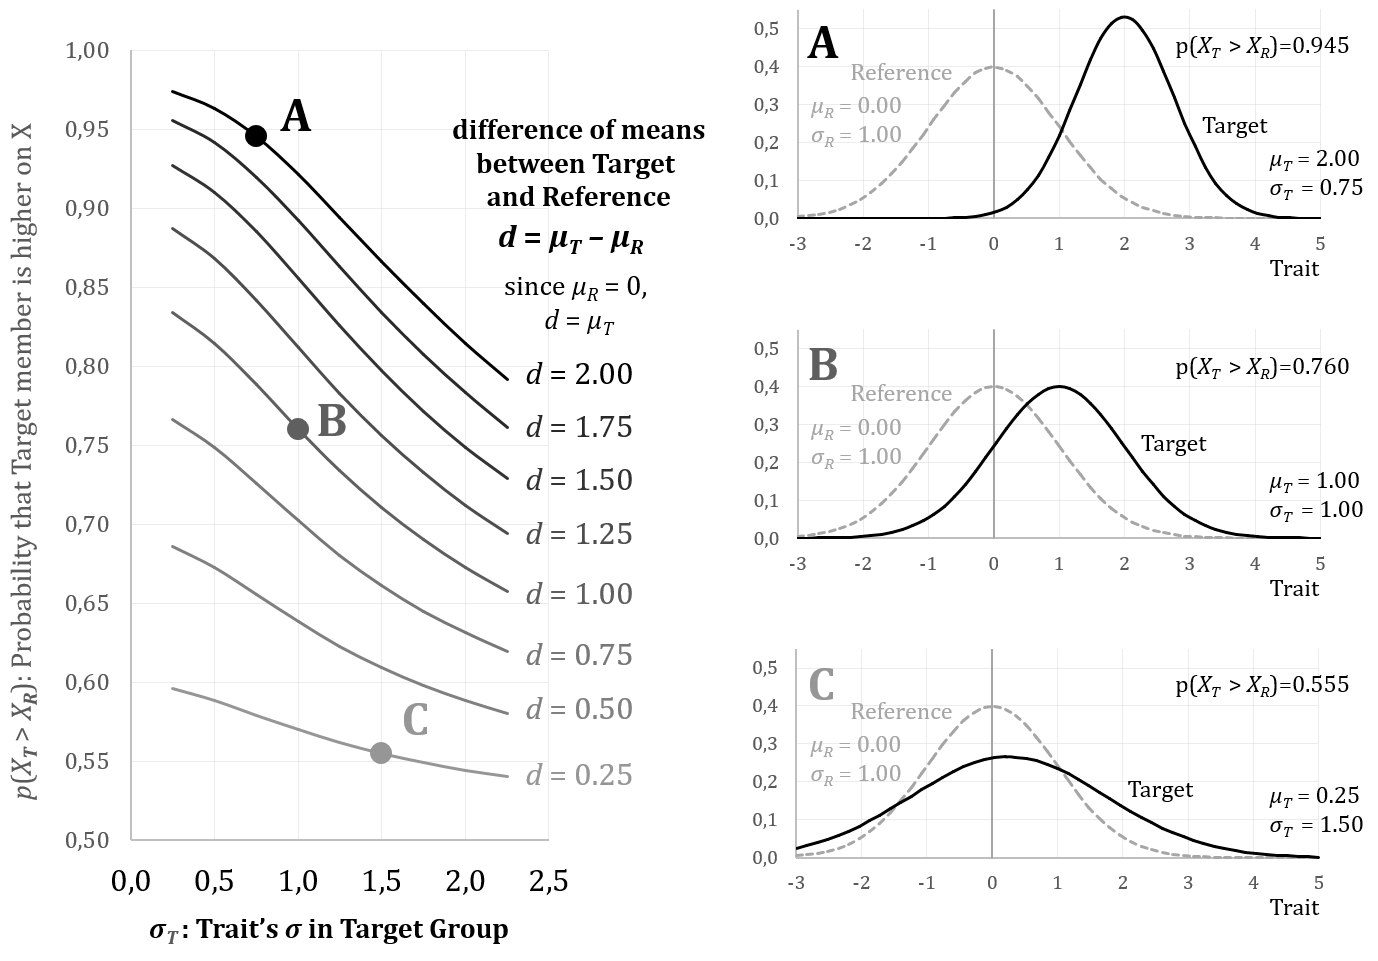
\includegraphics[width=\textwidth]{ART_Czarnik/Czarnik-img009.jpg}
\caption{Probability of a stereotype being true depending on the overlap of the trait's distributions in the target and reference group.}\label{fig1-czar}
\end{figure}



To make the link between the probability that \(X_{T} > X_{R}\) and the
relative location of the two distributions more intuitive, three
situations have been singled out for inspection:

\begin{flushleft}
\begin{enumerate}[label=\Alph*)]
\item
  \(\mu_{T} = 2.00\) and \(\sigma_{T} = 0.75\), with the corresponding
  \(p\left( X_{T} > X_{R} \right) = 0.945\);
\item
  \(\mu_{T} = 1.00\) and \(\sigma_{T} = 1.00\), with the corresponding
  \(p\left( X_{T} > X_{R} \right) = 0.760\);
\item
  \(\mu_{T} = 0.25\) and \(\sigma_{T} = 1.50\), with the corresponding
  \(p\left( X_{T} > X_{R} \right) = 0.555\).
\end{enumerate}
\end{flushleft}
In A, the stereotype could be considered to be very accurate as it would produce mistakes when judging individuals only 5.5\% of the time. In C, it is barely acceptable, with failure rate at 44.5\%. What about B? With the error rate at 24\% it seems quite unreliable. But before discarding it as a far-fetched overgeneralization, one should recognize that according to a popular metric proposed by Cohen
%\label{ref:RNDI9cG7tk2qD}(Cohen, 1988),
\parencite*[][]{cohen_statistical_1988}, %
 this stereotype signifies a definitely large effect size. With Cohen's \textit{d} equal to 1, it is the kind of effect that any social scientist would be more than happy to find in his or her study. Moreover, let us bear in mind that for ``new areas of research inquiry,'' effect sizes of 0.2 would not be utterly uninteresting 
%\label{ref:RNDDeitIcl8zR}(Cohen, 1988, p.25).
\parencite[][p.25]{cohen_statistical_1988}. %
 And it is just the effect size of a stereotypic difference depicted by C. Why should we then subject stereotypes to higher standards of truth than scientific findings?

For continuous variables, \(p\left( X_{T} > X_{R} \right)\) may be taken
directly as an unambiguous measure of the stereotype's accuracy because
probability that both individuals will happen to have equal values on X
equals zero. Thus if we fail to observe \(X_{T} > X_{R}\), the reverse,
\(X_{T} < X_{R}\), will be true. This is emphatically not the case with
discrete variables. The smaller the number of categories on the trait
variable, the more likely it is that the two individuals will be
indistinguishable with regard to X. The number of \(X_{T} = X_{R}\)
pairs will grow at the expense of both \(X_{T} > X_{R}\) and
\(X_{T} < X_{R}\).

Figure \ref{fig2-czar} illustrates the effect of categorization on the probabilities. Three simulations were done, each involving 100 ``persons'' (50 from the target group, and 50 from the reference group). Each group of 50 values constituted a representative selection from the underlying continuous distribution with standard deviation equal to 1. In terms of Cohen's \textit{d}, simulation no. 1 exemplified a moderate size effect ( $\mu _T-\mu _R=0.5$), simulation no. 2 a large effect ( $\mu _T-\mu _R=1.0$), and simulation no. 3 a very large one ( $\mu _T-\mu _R=1.5$). In each case, 100 values from both groups were jointly ranked and grouped into 20 categories, then into 19, then 18, and so on until the final rough division into two categories: those above and those below the median. With the original continuous variables, the probabilities $p\left(X_T>X_R\right)$ were 0.64, 0.77, and 0.87 for moderate, strong, and very strong effect sizes, respectively (see the black bullet markers in Figure \ref{fig2-czar}). These probabilities decrease systematically, even though very slightly at first, with the ongoing reduction in the number of categories. Serious distortions occur when the distributions are reduced to three or, especially, two categories.\footnote{For example, $p\left(X_T>X_R\right)=0.87$ associated with a very large effect on a continuous trait, dwindles to 0.61 after reducing the trait to a dichotomy—still noticeable but far from impressive.} $X_T=X_R$ probabilities are steadily on the rise, and for the moderate effect ( $\mu _T-\mu _R=0.5$), we observe that splitting the continuum into two parts even makes $X_T=X_R$ the most likely outcome. On the positive side, probabilities are not that heavily affected by reduction to five categories—the number of points on a Likert-type scale routinely applied to measure attitudes in surveys.


\setlength{\tabcolsep}{2pt}
\begin{figure}[H]
	\begin{small}
   \begin{supertabular}{m{.32\textwidth}m{.32\textwidth}m{.32\textwidth}}
   \begin{center}
   \textbf{moderate effect size}
   \end{center} &
   \begin{center}
   \textbf{large effect size}
   \end{center} &
   \begin{center}
   \textbf{very large effect size}
   \end{center} \\
	\vskip-.3in$$\mu_{T} - \mu_{R} = 0.5$$\vskip-.3in &
    \vskip-.3in$$\mu_{T} - \mu_{R} = 1.0$$\vskip-.3in &
    \vskip-.3in$$\mu_{T} - \mu_{R} = 1.5$$\vskip-.3in \\
   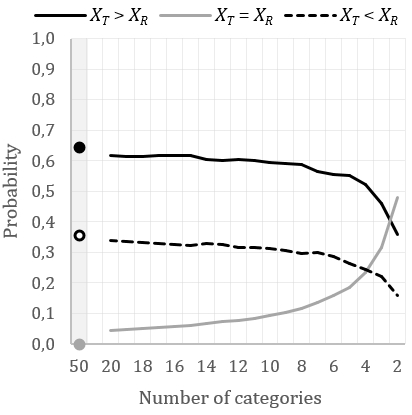
\includegraphics[width=\linewidth]{ART_Czarnik/Czarnik-img016.jpg} &
   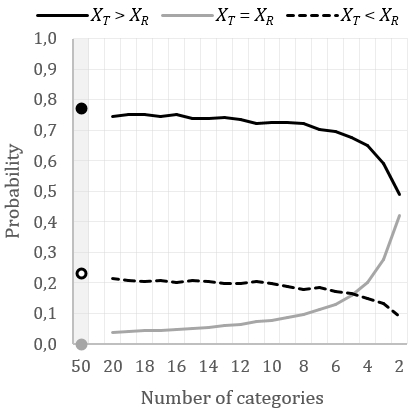
\includegraphics[width=\linewidth]{ART_Czarnik/Czarnik-img017.jpg} &
   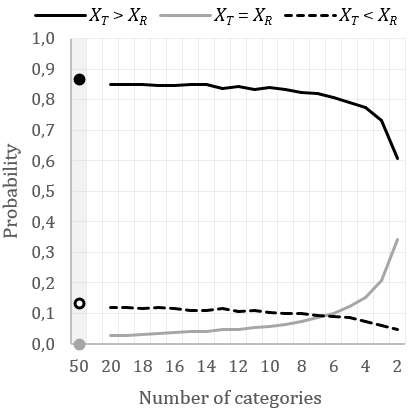
\includegraphics[width=\linewidth]{ART_Czarnik/Czarnik-img018.jpg} \\
   \end{supertabular}
   \end{small}
\caption{The effect of categorization on the observed
probabilities of \(X_{T} > X_{R}\), \(X_{T} = X_{R}\), and
\(X_{T} < X_{R}\) for three different effect sizes (all underlying
distributions are normal with \(\sigma_{T} = \sigma_{R} = 1\)).}\label{fig2-czar}
\end{figure}
When analyzing the accuracy of stereotypes regarding traits measured on
scales with a limited number of categories it is thus advisable to
consider all three possible options: \(X_{T} > X_{R}\),
\(X_{T} = X_{R}\), and \(X_{T} < X_{R}\)\footnote{The effect of categorization cannot be held constant by using the contrast between $p(X_T>X_R)$ and $p(X_T<X_R)$ as a measure. The difference $p(X_T>X_R)-p(X_T<X_R)$ tends to decrease, and the ratio $p(X_T>X_R)\ /\ p(X_T<X_R)$ tends to increase as the number of categories becomes smaller and smaller.}, as it may well turn out that
\(p\left( X_{T} = X_{R} \right)\) is far from negligible.
\enlargethispage{1\baselineskip}

\section{A few empirical examples of assessing the accuracy of sex stereotypes}
Both actual differences between the sexes and associated beliefs about these differences were intensively studied
%\label{ref:RND1zeV4PeuSF}(Williams and Best, 1982, 1990; Costa, Terracciano and McCrae, 2001; Biernat and Deaux, 2000; Buss, 2003; Pinker, 2003).
\parencites[][]{williams_measuring_1982}[][]{williams_sex_1990}[][]{costa_gender_2001}[][]{borgatta_sex_2000}[][]{buss_evolution_2003}[][]{pinker_blank_2003}. %
 In the following, I~will examine a number of possible sex stereotypes, testing their accuracy against the survey data from Polish General Social Survey 
%\label{ref:RNDDqAxDLuyEC}(Cichomski, Jerzyński and Zieliński., 2013)
\parencite[][]{cichomski_polskie_2013} %
 and the Study of Human Capital in Poland 
%\label{ref:RNDLH293GzyiT}(Górniak et al., 2015, 2019).
\parencites[][]{gorniak_bilans_2015}[][]{gorniak_bilans_2019}.%
\footnote{Representative surveys provide us with proper criteria for assessing stereotypes' accuracy. } It is irrelevant here whether most people (or any people, for that matter) subscribe to these particular stereotypes, although certainly some of the inspected traits are popularly held to be gender-differentiating (e.g. body height, earnings, interest in fashion or technology).

For each trait, probabilities of a randomly selected woman being at a
higher, the same, or lower level on the trait as compared to a randomly
selected man were computed, using the following formulae, where \emph{v}
stands for a value of the trait variable\footnote{It may be noted that a
  difference between the ``mirror-image'' probabilities, i.e.
  \(p\left( X_{F} > X_{M} \right) - p\left( X_{F} < X_{M} \right)\),
  is equal in value to asymmetric Somer's \textit{d} rank correlation coefficient
  \parencite{somers_new_1962}, when predictions are based on subjects' sex.}:
\[p\left( X_{F} > X_{M} \right) = \sum_{v = min}^{\max}{p\left( X_{F} = v \right) \cdot p\left( X_{M} < v \right)}\]

\[p\left( X_{F} = X_{M} \right) = \sum_{v = min}^{\max}{p\left( X_{F} = v \right) \cdot p\left( X_{M} = v \right)}\]

\[p\left( X_{F} < X_{M} \right) = \sum_{v = min}^{\max}{p\left( X_{F} = v \right) \cdot p\left( X_{M} > v \right)}\]

Figures \ref{fig3-czar} to \ref{fig6-czar} summarize the results.

\begin{figure}[H]
	\centering
   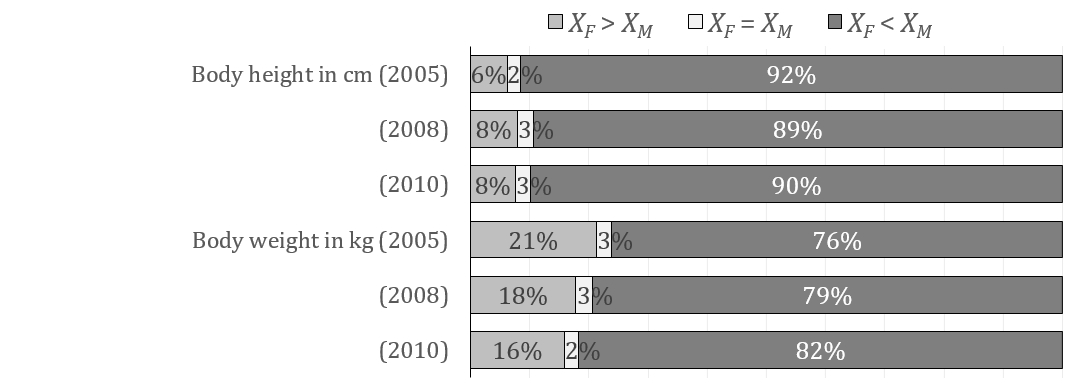
\includegraphics[width=\textwidth]{ART_Czarnik/Czarnik-img019.jpg}
\caption{Probabilistic assessment of stereotypical sex differences concerning body structure.\\
{\footnotesize Own computation from Polish General Social Survey data elicited by open-ended questions
``What is your height and weight, approximately?''}. 
}\label{fig3-czar}
\end{figure}


Both height and weight are near-continuous variables and therefore it's very unlikely that the two randomly selected individuals will be of the same height or weight. The probabilistic differential is very large indeed, especially with regard to height. Thus the ``men are taller than women'' stereotype will hold true for about 90\% of the randomly matched male-female pairs. It is about 12 times more likely that a man will be the taller of the two than the other way round.

\begin{figure}[H]
	\centering
   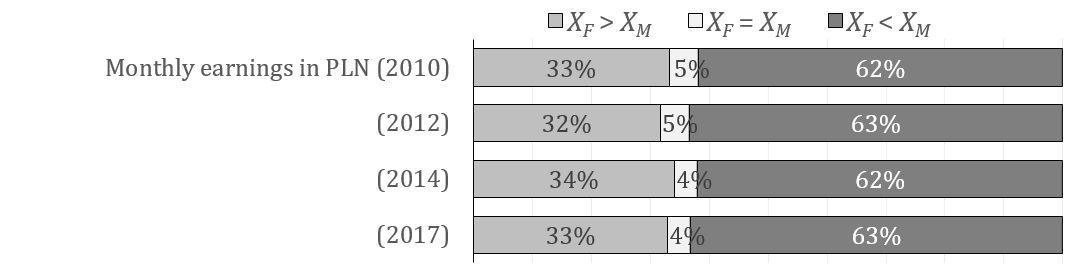
\includegraphics[width=\textwidth]{ART_Czarnik/Czarnik-img020.jpg}
\caption{Probabilistic assessment of stereotypical sex differences concerning pay.\\
{\footnotesize Own computation from the Study of Human Capital in Poland data elicited by open-ended questions with supplementary categorization (analysis restricted to employees with job contracts working full-time within last month, excluding self-employed).  }
}\label{fig4-czar}
\end{figure}

Sex difference in average remuneration, widely publicized under the heading of ``gender pay gap'', is common knowledge these days. However, the stereotypic assertion that men earn more than women is a rule with quite a lot of exceptions. In Poland, it is correct for more than 60\% of the random individual comparisons, yet every third time the reverse is true. Interestingly, hardly anybody is prompted by such substantial amount of ``counterevidence'' to dismiss male-female wage differential as a mere stereotype.\footnote{Similarly, Browne
%\label{ref:RNDKyToDmIZds}(1998)
\parencite*[][]{browne_divided_1998} %
 observes that while temperamental differences between the sexes (e.g. in competitiveness and risk-taking) are likely to be brushed aside because they ``do not hold true for all individuals'', the very same argument is hardly ever used to shrug off the economic differences. } On the contrary, the issue is widely researched, prominent in political agendas, and dealt with in antidiscrimination legislation.

\begin{figure}[H]
	\centering
   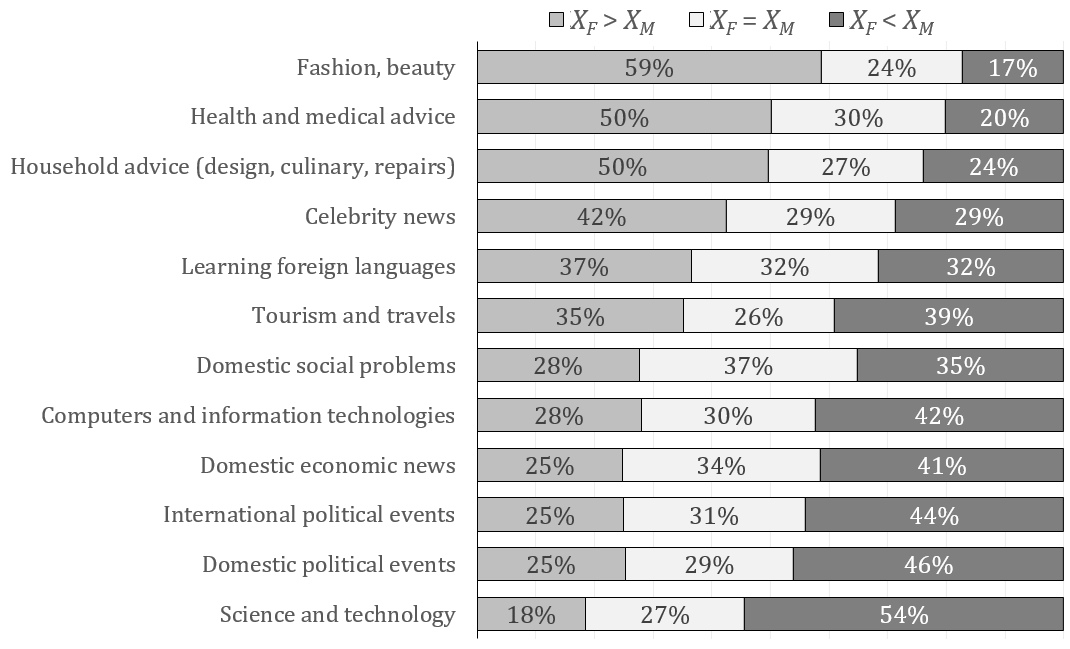
\includegraphics[width=\textwidth]{ART_Czarnik/Czarnik-img021.jpg}
\caption{Probabilistic assessment of stereotypical sex differences concerning interest in the mass media content.\\
{\footnotesize Own computation from Polish General Social Survey data (2002). Interest was measured on a 4-point scale: 1 not at all /2 not much /3 quite a bit /4
very much.}
}\label{fig5-czar}
\end{figure}

In Figure \ref{fig5-czar}, people's interests are sorted by gender differences, from those most typical of women at the top to those most typical of men, at the bottom. Some of those differences are congruent with popular sex stereotypes (e.g. those concerning fashion or technology), but even then many exceptions arise. As may be expected for traits measured using categorical scales, a substantial number of male-female comparisons produce gender-equal outcomes. Still, it is unsurprising why someone seeking medical advice from a random stranger would turn for help to a woman rather than a man. As far as a man and a woman differ in their levels of medical interests and as far as the intensity of such expressed interests is proportional to actual cognizance, it is a woman who is about 2.5 times more likely to have some acquaintance with health topics. By the same token, if one seeks technological advice, it's three times more likely that of any two random strangers, one man and one woman, the man will be the one more up-to-date with matters of technology.

\begin{figure}[h]
	\centering
   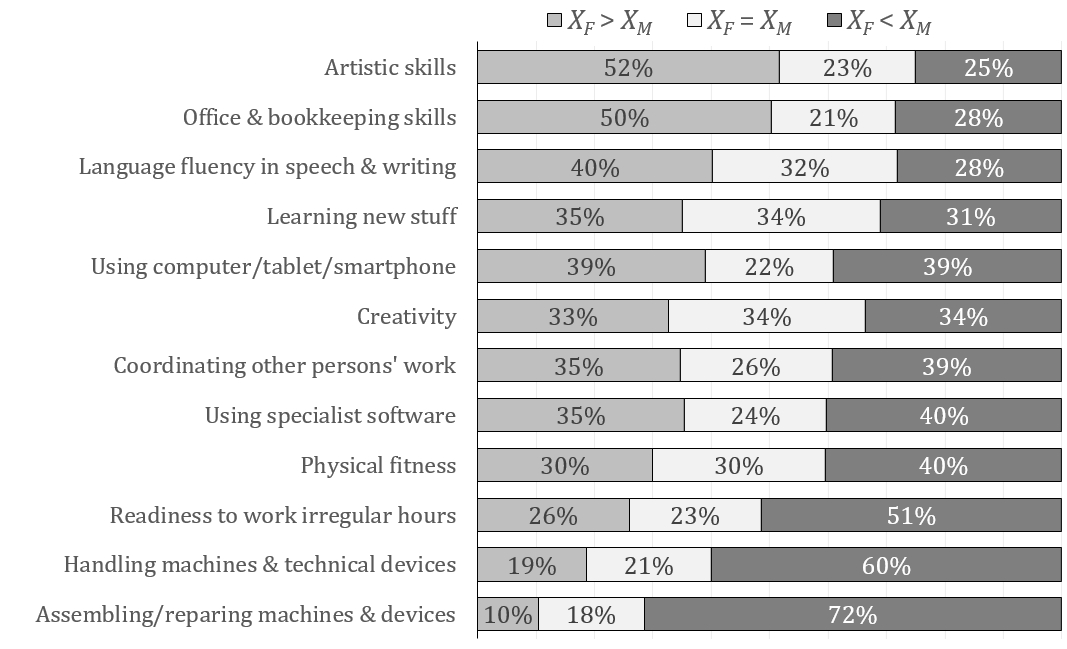
\includegraphics[width=\textwidth]{ART_Czarnik/Czarnik-img022.jpg}
\caption{Probabilistic assessment of stereotypical sex differences concerning skill self-evaluation.\\
{\footnotesize Own computation from the Study of Human Capital in Poland data (2017). Skill level was self-evaluated on a 5-point scale: 1 low /2 basic /3 medium /4 high /5 very high.}}\label{fig6-czar}
\end{figure}

One can observe that stereotypical disparities in skill self-evaluations are in accord with the kinds of jobs men and women tend to perform in the gender-segregated labor market
%\label{ref:RNDeyzjhDc1o6}(Czarnik and Kasparek, 2015).
\parencite[][]{czarnik_gender_2015}. %
 The probabilistic skill differentials are most pronounced in the areas heavily dominated by either sex, i.e. clerical jobs associated with office and bookkeeping skills (women) and jobs in industry, construction, and transportation involving machines and technological environment (men). On the other hand, we see that ``men perceive themselves to be natural managers'' kind of stereotype is true by such a thin margin that it's hardly worth mentioning (see ``Coordinating other persons' work'').

\section{How good are people in assessing accuracy of stereotypes?}
As shown above, stereotypic assertions in their generic formulation may vary substantially in how much truth they contain when applied at individual level and it would be very foolish of stereotype holders, namely all of us, not to recognize the fact. Fortunately, as Schneider
%\label{ref:RNDFOmE4JC32O}(2005, p.199)
\parencite*[][p.199]{schneider_psychology_2005} %
 put it, ``[n]ot always, to be sure, but still most of us are aware that stereotypes are only probabilistically true and do not apply to everyone.'' And even if it was true, as Pinker 
%\label{ref:RND9JKr0iPkC4}(2007, p.86)
\parencite*[][p.86]{pinker_stuff_2007} %
 claims, that ``[t]he image of one orb floating above another seems to come more naturally to the mind than an image of two overlapping bell curves'', people are capable of implicitly processing this kind of information to arrive at probabilistic statements. They may commit a number of mistakes in the process, as observed by Whitley and Kite 
%\label{ref:RND7JZzDeXpJE}(2010, p.100):
\parencite*[][p.100]{whitley_psychology_2010}:%


\myquote{
Research participants might be fairly accurate, for example, in their estimates of what percentage of Asians are mathematical, but they might be inaccurate in their estimate of the variability of this characteristic. If perceivers are accurate on one measure, but not the other, does their belief have a kernel of truth? This question is difficult to answer.
}

Yet this question \textit{can} be answered by applying the probabilistic approach. It is even more to the point for the very reason that it is our probabilistic beliefs that inform our decisions concerning individuals. A typical question you would ask yourself when pressed to choose, with certain aim in mind, one from two or more persons would not be ``what is the difference of means between the groups to which these persons belong?'', and even less ``how large is the dispersion of the relevant characteristic?''. It would be ``which one of them is most likely to give me what I need?''. This probabilistic perception can easily be measured by asking people to imagine a familiar situation and make the assessment of comparative probabilities. By means of an illustration, consider how subjects could assess the accuracy of the stereotypic ``men are taller than women'' assertion.

\myquote{
Imagine that you enter an elevator in a large shopping mall and two random persons—one man and one woman—unacquainted to you and to each other,\footnote{It is important to exclude the possibility that a man and a woman are a couple, so that subjects' judgment about general differences would not be contaminated by their beliefs about relative height of mated individuals. } enter after you. How likely it is that: (1) the man will be the taller of the two, (2) the woman will be the taller of the two, (3) they will be of equal height (with precision of, say, 1 cm). Make sure that probabilities add to 100\%.\footnote{It is a subject for some experimentation to find out how this task could be facilitated by a particular method of registering the probabilities (e.g. by a visual representation of probabilities on screen). }
}

A very welcome aspect of this approach is that it explicitly tackles the question of whether subjects' beliefs about certain group(s) of people are of a rigid, all-or-none, kind. This should provide solid empirical evidence to inform the dispute over sensibility of making stereotypes untrue by definition. In all likelihood, for many traits it will turn out that actually very few people incorrectly perceive the stereotyped group(s) as completely homogeneous.

Subjective probabilities elicited in this way could then be compared to the factual probabilities calculated from the source data, e.g. representative survey. For example, in the particular case of the male-female height comparison, my educated guess—informed by a number of informal trials—would be that people tend to \textit{under}estimate the accuracy of the height stereotype.

To be sure, we still should be cautious not to make too much of such evidence. It is entirely plausible that even if people make nuanced probabilistic judgments when explicitly prompted to make them, they can still—especially in the absence of such prompts—behave automatically and unreflectively fall prey to the rigid all-or-nothing kind of thinking when making their everyday decisions. I think that an especially worthwhile avenue for further research is to investigate the relationship between the perceived accuracy of a given stereotype and perceiver's openness to, or even active seeking of, individuating information when making decisions.

\section{Conclusion}
Since the introduction of the concept into academic realm, a topic of stereotype accuracy was and remains controversial. As negative stereotypes have been linked to prejudice and discrimination, it seemed justified to view stereotypic beliefs as anything but accurate depictions of reality. However, this wholesale dismissal, insofar as it extends to all perceptions of group differences, has serious disadvantages. First, the larger the actual differences between the groups, the more obvious it is that the stereotype is (to some extent) accurate, and all statements to the contrary sound deceitful. In effect, all efforts at eradicating demonstrably false stereotypes may be hindered, as the criticism of stereotypes will lose its \textit{prima facie} credibility. Second, outright denial of group differences where they do exist and contribute to the perceived inequality between groups severely restricts the repertoire of actions that could be taken to address the problem.

Even if many group differences turn out to be real rather than imaginary, bigots—to reiterate Kenny
%\label{ref:RND84Zh1FAM8u}(Kenny, 1994, p.212)
\parencite*[][p.212]{kenny_interpersonal_1994}%
—``should not take any comfort in these conclusions.''\footnote{Bigots should also be well advised to recognize that they themselves are a strongly stereotyped group, and these stereotypes may turn out to be not so far from the truth, either. } Such differences leave space—in some instances a whole lot of space—for exceptions. They also evolve: they may grow bigger, but equally likely they may grow smaller, vanish or even be reversed. In any case, to minimize the stereotype-based discrimination, it is always advisable to advocate the individualistic approach, i.e. to explain why the best decisions are the ones based—whenever possible and to whatever extent feasible—on person's individual characteristics rather than on the average characteristics of the groups individuals belong to.

Testing stereotype's accuracy in probabilistic terms has a direct advantage of bridging the gap between collective and individual levels of analysis, both of which are explicitly involved in making probabilistic comparisons. This, to satisfy Jussim
%\label{ref:RNDerlUautrYn}(2012, p.309),
\parencite*[][p.309]{jussim_social_2012}, %
 should bring ``greater conceptual clarity […] to understanding stereotype accuracy.'' It could also be a step towards meeting concerns voiced by Stangor 
%\label{ref:RNDs3zgPwUmNI}(1995, p.278)
\parencite*[][p.278]{lee_content_1995} %
 that in order to find ``an adequate remedy for negative intergroup behavior […] We need to know both how big existing group differences are and how to communicate the extent of those differences to people.'' It seems that probabilistic approach is quite a promising avenue in this regard by explicitly bringing up counterexamples to the stereotype under question.

In the end, no matter how much—or how little—truth any particular stereotypes may contain, ``what matters is […] the gullibility with which we employ them''. And we would be wise indeed to take this advice from Walter Lippmann, which is no less prudent today than it was a hundred years ago:

\myquote{
if our philosophy tells us that each man is only a small part of the world, that his intelligence catches at best only phases and aspects in a coarse net of ideas, then, when we use our stereotypes, we tend to know that they are only stereotypes, to hold them lightly, to modify them gladly
%\label{ref:RNDTWIiYL2CPo}(Lippmann, 1998, pp.90–91).
\parencite[][pp.90–91]{lippmann_public_1998}.%
}


\paragraph{Acknowledgment}
Insightful comments by two anonymous reviewers and a mathematical consultation from Dr. Paweł Hołobut (IPPT PAN) are gratefully acknowledged.

\end{artengenv}
